\documentclass{scrartcl}

\usepackage{tikz}
%\usetikzlibrary{trees,snakes}
\usetikzlibrary{plotmarks,mindmap}
\usetikzlibrary{arrows, positioning, shadows, backgrounds, scopes, positioning}
\usepackage{verbatim}
\usepackage{enumerate, amsmath, amssymb,amsthm, amstext}

\begin{document}

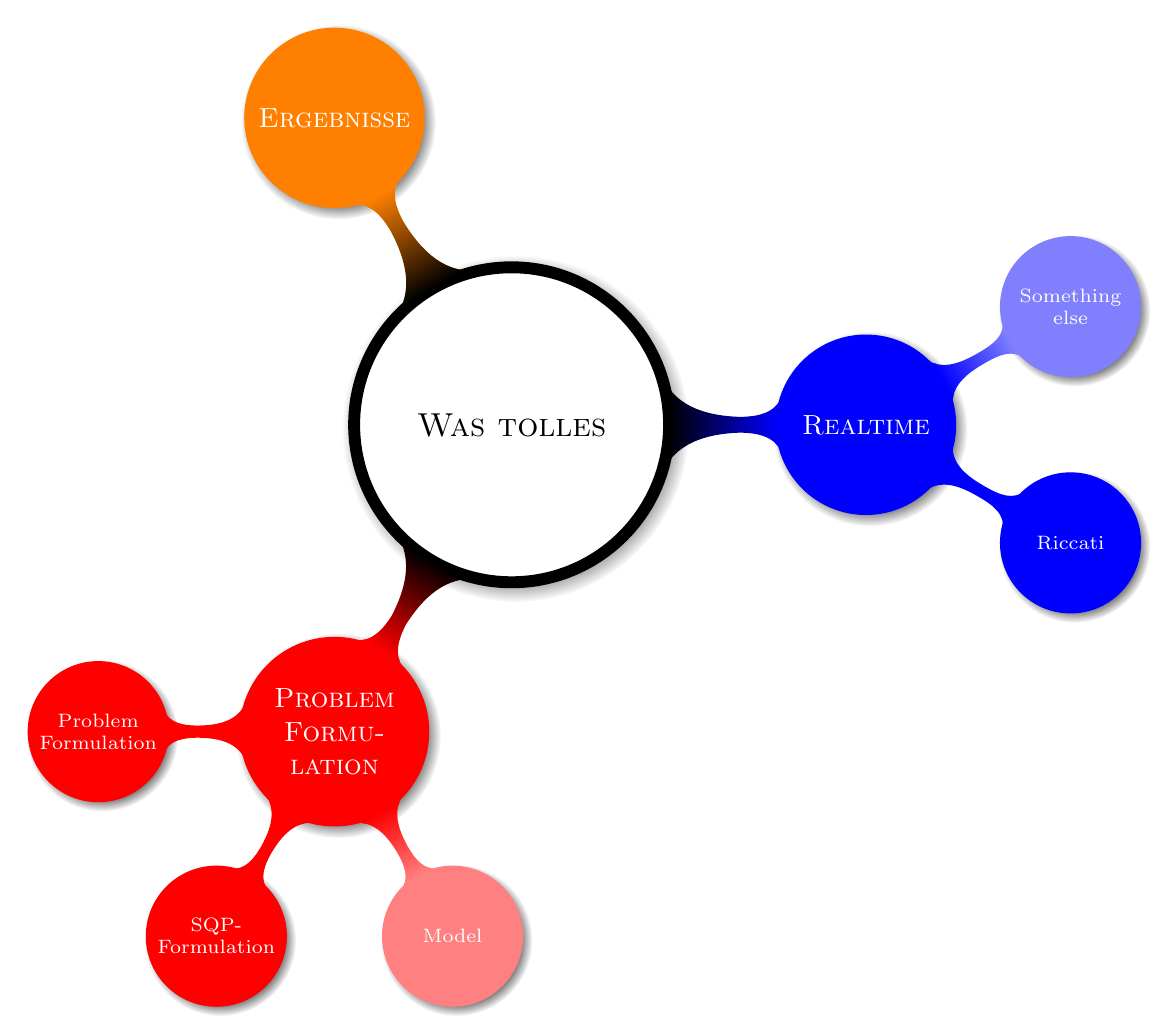
\begin{tikzpicture}[mindmap]
\begin{scope}[
every node/.style={concept, circular drop shadow,execute at begin node=\hskip0pt},
root concept/.append style={
concept color=black, fill=white, line width=1ex, text=black, font=\large\scshape},
text=white,
computational problems/.style={concept color=red,faded/.style={concept color=red!50}},
computational models/.style={concept color=blue,faded/.style={concept color=blue!50}},
measuring complexity/.style={concept color=orange,faded/.style={concept color=orange!50}},
solving problems/.style={concept color=green!50!black,faded/.style={concept color=green!50!black!50}},
grow cyclic,
level 1/.append style={level distance=4.5cm,sibling angle=120,font=\scshape},
level 2/.append style={level distance=3cm,sibling angle=60,font=\scriptsize}]
\node [root concept] {Was tolles} % root
child [computational problems] { node {Problem Formulation}
child { node {Problem Formulation} }
child { node {SQP-Formulation} }
child [faded] { node {Model} }
}
child [computational models] { node {Realtime}
child { node {Riccati} }
child [faded] { node {Something else} }
}
child[measuring complexity] {node {Ergebnisse}}
;
\end{scope}
\end{tikzpicture}

\end{document}